\section{Architecture}
\label{sec:architecture}

A criminal network analytics application requires real-time processing of heterogeneous data from multiple distributed sources, as mentioned in the previous sections.

In an international level criminal scenario, the amount of data that must be managed reaches considerable size: a large number of people, criminals, devices, and sensors are connected via digital networks, and the cross plays among these entities generate enormous valuable information\cite{FrameworkBigdata}. For these reasons, we are interested to an high-throughput and scalable process of analysis, based to the input data rate.
Furthermore, application usage as a tool to support the law enforcement agencies, it requires the storage capacity of the social network in a database that can be consulted rapidly.

Considering these requirements, in this research we prorpose an application that follow a \textit{data stream processing(DSP)} approach. DSP is a computational paradigm in which the sources, called \textit{stream}, emit continuous data flows, which are then processed in real time by distributed and parallelized operators. Our application uses \textit{Apache Flink}\cite{flink} as a data stream processing framework 

Data aggregation is provided by \textit{Apache Kafka}\cite{kafka}, an high-throughput message queuing system, designed for making streaming data available to consumer (Flink in our case). Kafka makes the streaming data by durable persisting incoming messages on disk, using a date structure log, and implements a \textit{publish/subscribe} mechanism to \textit{asynchronous communication} of data to Flink.

Criminal network's graph is stored in \textit{Neo4j}\cite{neo4j}. Neo4j is a highly scalable, native graph database purpose-built to leverage not only data but also its relationships. We chose Neo4j because apart from being specific for problem, it allows interactive viewing of the graph through a webpage.
In figure \ref{fig:toplogy} we represent the topology of architecture implemented with Flink and the interactions with Kafka and Neo4j.

In figura 2 la topologia dell'architettura realizzata su Flink, e l'interazione con Kafka e Neo4j. Both mining techniques are performed in parallel. Scores are filtered with a thresholding process and the output is the set of hidden links and potential links, available on the webpage of Neo4j and Flink's log.
 
%\begin{figure}[]
%	\centering
%	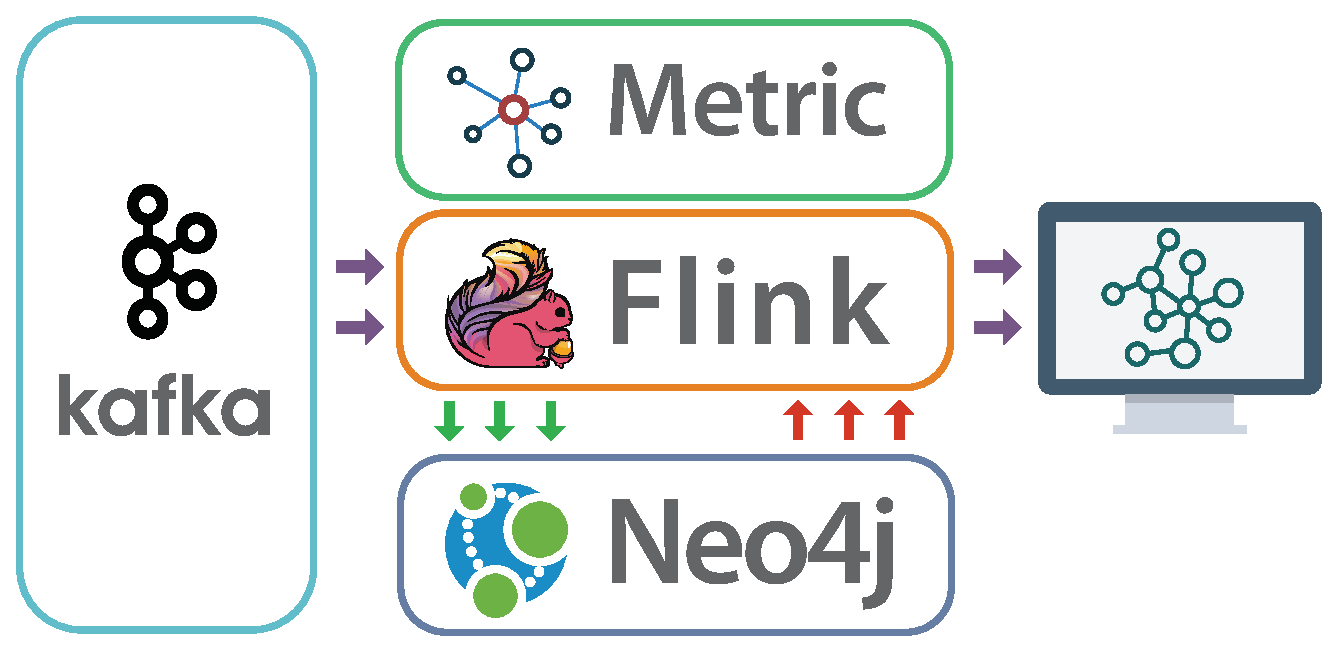
\includegraphics[width=0.48\textwidth]{fig/crimegraph-layered-architecture.eps}
%	\caption{High-level architecture.}
%	\label{fig:layered-architecture}
%\end{figure}


In Figure~\ref{fig:architecture}

\begin{figure*}
\centering
\includegraphics[width=6in]{./fig/topology}
\caption{The topology of architecture.}
\label{fig:toplogy}
\end{figure*}

